\begin{figure}[!ht]
    \centering

    \begin{subfigure}{1\linewidth}
        \centering
        
\includegraphics[width=0.45\linewidth]{anisoglints/anisobrdf.png}
        
\includegraphics[width=0.45\linewidth]{anisoglints/anisostretched.png}
        \caption{Anisotropic dielectric plane}
    \end{subfigure}

    \begin{subfigure}{1\linewidth}
        \centering
        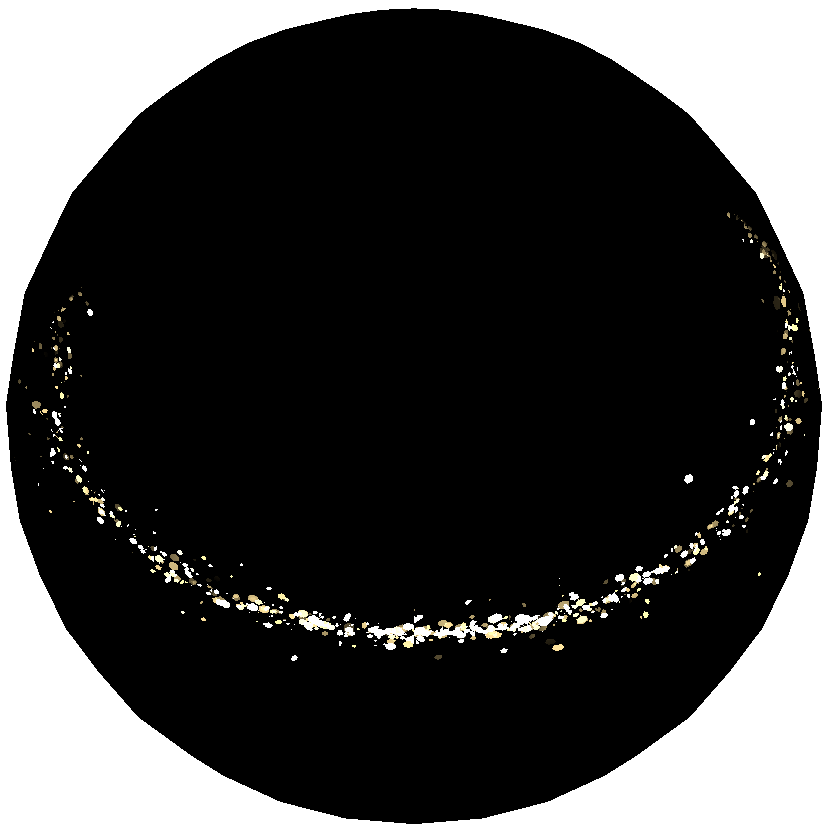
\includegraphics[width=0.4\linewidth]{anisoglints/anisobrdfball.png}
        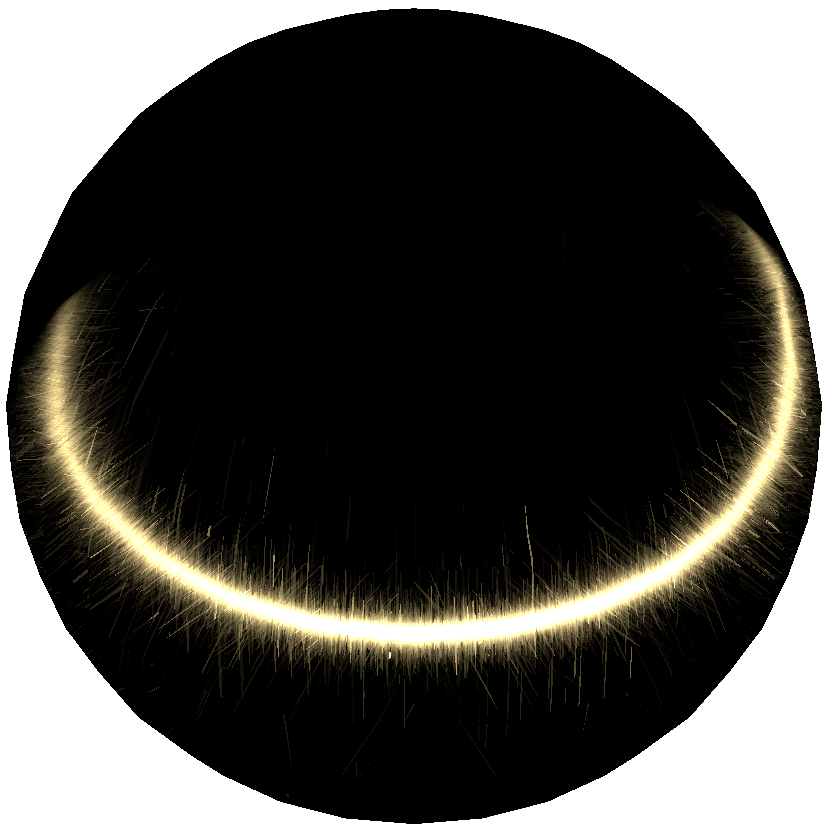
\includegraphics[width=0.4\linewidth]{anisoglints/anisostretchedball.png}
        \caption{Anisotropic gold ball}
    \end{subfigure}

    \caption{Two different objects rendered using an anisotropic base BRDF, with a symmetric surface grid (left) and stretched surface grid (right) respectively. One can notice that the glints are incorrectly aligned especially at the sides. This occurs because of the non-uniform anisotropy compensating surface parametrization.\label{fig:anisoglints}}
\end{figure}